\section{Results}
The application of the \Ex MPM solver to simulate membrane compaction is discussed in this section. 

%A few words about the experiments
The membrane compaction experiment to be simulated in MPM is chosen from \cite{WU2022115875}. In the cited article, the authors have chosen an HPRO (XUS1818, Dupont Water Solutions, Edina, Minnesota, USA) membrane to perform experimental studies on its flux and salt rejection properties. The membrane is subjected to high (14 bar) and ultra-high pressures (200 bar) using pressurized N2 gas. After the application of pressure, a sample of the membrane is analyzed for its pore structures in an SEM. The original and compressed membrane heights are available for MPM validation.

%Modeling challenges.
One of the primary challenges in modeling the membrane compaction experiment using MPM is to obtain the initial material point locations. Due to the intricate and minute pore structures, detailed computer-aided modeling of the membrane is next to impossible. In this study, the initial material points are generated  from the images obtained from SEM. Already existing Python modules are used to read the SEM image file. Once the image file is read by the python script into an array, it is converted into grayscale. Since the objective here is to identify and represent only the larger microvoids in the membrane, image intensity-based filtering is performed. Based on trial and error, the image is clipped between intensities $20$ and $180$ to obtain a good representation of the membrane. Each pixel in the clipped image is then treated as a material point. The dimensions of the membrane are calibrated such that the entire membrane height is kept close to 50 microns. For ease of computation, the membrane geometry is assumed to be periodic, and only one layer of material points is retained in the third dimension. The top row in Figure~\ref{fig:expt_mpm_compare} shows the SEM image and the material point locations used in this study.

\begin{figure}[tbh]
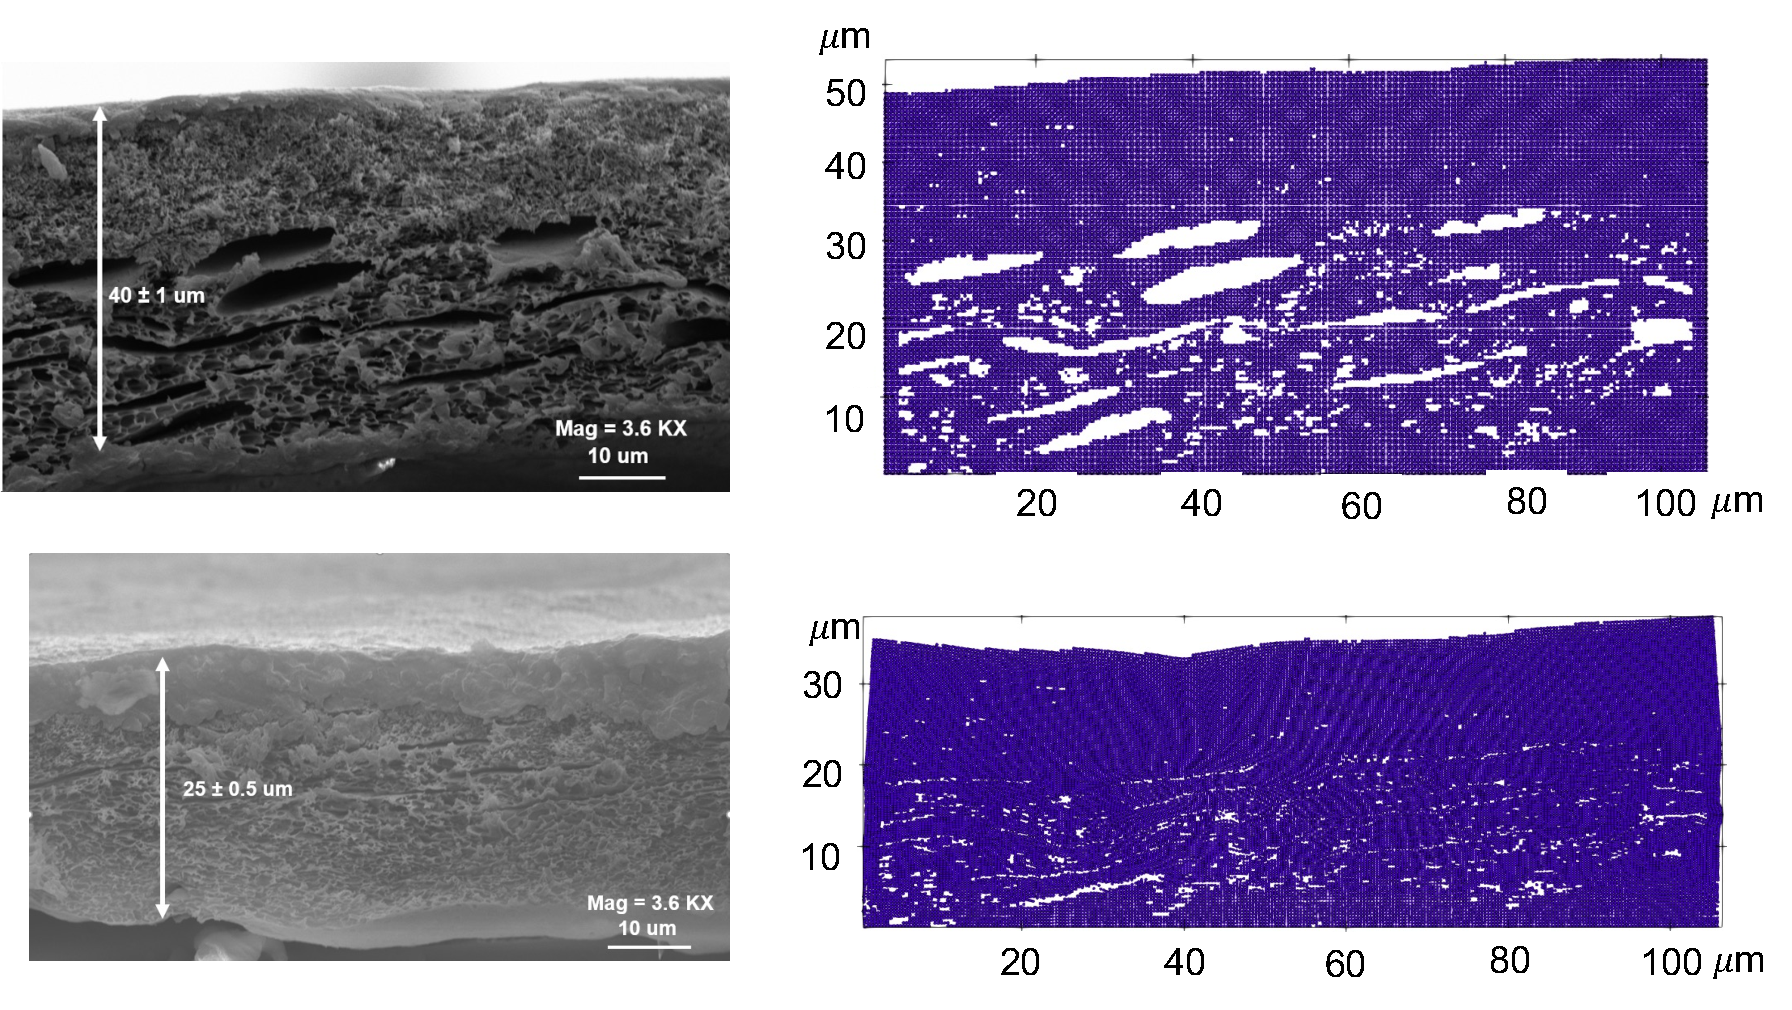
\includegraphics[width=\textwidth]{./PICS/compare_expt_mpm.pdf}
\caption{(top left) and (top right) show SEM image of PSF layer and corresponding material point representation that is used as initial condition for our simulations. (bottom left) and (bottom right) show SEM image of compressed PSF layer at 200 bar pressure and corresponding snapshot of material points at steady state for a compression simulation at 200 bar.}
\label{fig:expt_mpm_compare}
\end{figure}

%Problem setup
The PSF material in the membrane is modeled as a linear elastic material. The value of Young's modulus (134 MPa) is obtained from a tensile test carried out at the UCLA NanoMeTeR laboratory, and the Poisson's ratio is assumed to be $0.3$. The application of pressure (200 bar) on the membrane is modeled by applying a fictitious body force on the material points. The applied body force is calibrated such as to obtain an average normal stress equal to the imposed pressure. The boundary condition applied on the bottom surface of the background grid is that of a no-slip wall, while slip walls are applied on all the other boundaries. To maintain a low computational cost, the linear-hat function is used as the spatial scheme. The values of CFL and $\alpha_{P_F}$ are set as $0.1$ and $0.95$, respectively.


%
%Results
Simulation is carried out in an HPC environment with 2 GPU nodes. Figure~\ref{fig:stress}(a) shows the time evolution of the average normal stress in the y-direction on the top surface. It can be observed that the stress value recovers to  that of the imposed pressure indicating that the steady-state solution is attained. The bottom images in Figure~\ref{fig:expt_mpm_compare} show a comparison between the experimentally and numerically observed compacted membrane and their pore structure. Experiments report a membrane deflection of 15 microns (a strain of 0.375) while MPM results show a deflection of 17 microns (a strain of 0.34). An accurate prediction in terms of deflection is obtained with the deviation of MPM results from experiments being only 3.5\%. Figure~\ref{fig:stress}(b) shows the y-normal stress and the compacted configuration of the membrane. The figure shows the presence of microvoids now compressed under pressure, very similar in shape to that found in experiments. Regions of stress concentrations near the corners of the voids can also be observed.

\begin{figure}[tbh]
\centering
\begin{subfigure}[b]{0.49\textwidth}
    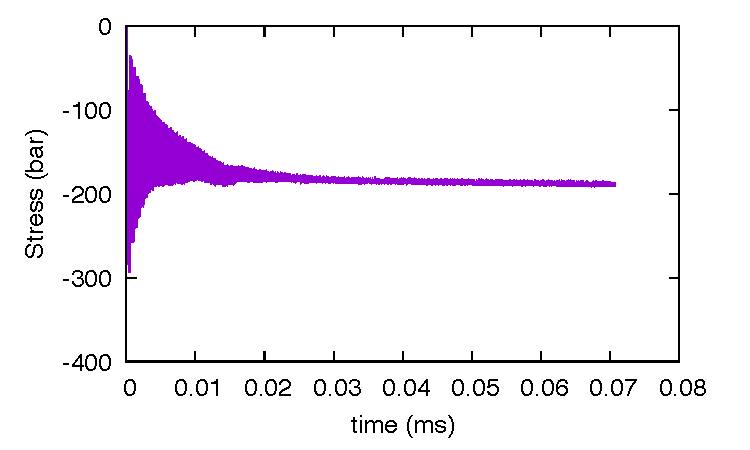
\includegraphics[width=0.99\textwidth]{./PICS/force.pdf}
    \caption{}
\end{subfigure}
\begin{subfigure}[b]{0.49\textwidth}
    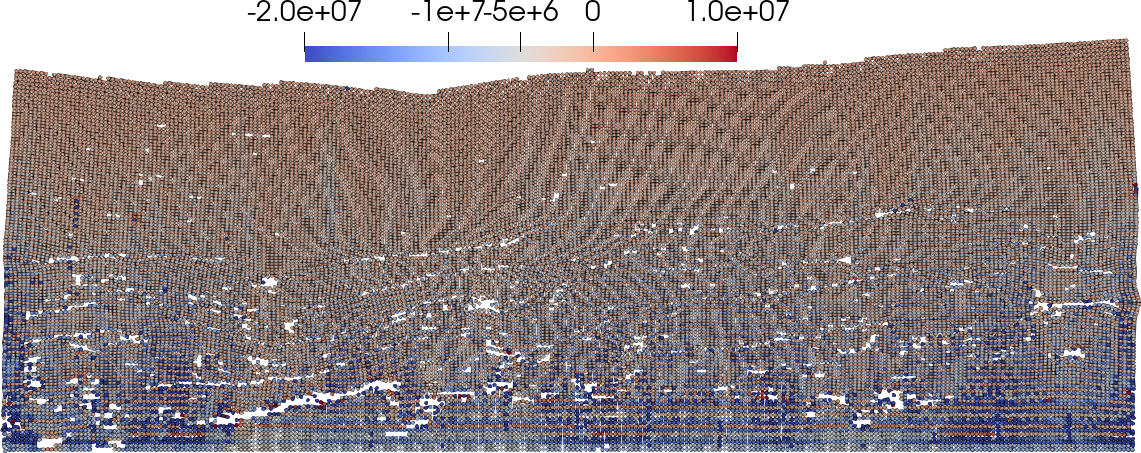
\includegraphics[width=0.99\textwidth]{./PICS/stress.png}
    \caption{}
\end{subfigure}
\caption{(a) average axial stress history at the bottom of the domain that tends to 200 bar at steady-state and (b) is the stress distribution in Pa among material points at steady-state.}
\label{fig:stress} 
\end{figure}